En esta sección se presenta la metodología de este trabajo tanto teórica como experimental. Partiendo desde la matemática del problema hasta la arquitectura de las redes neuronales utilizadas. En esta sección se presenta la metodología de este trabajo tanto teórica como experimental. Partiendo desde la matemática del problema hasta la arquitectura de las redes neuronales utilizadas. Se describen las variables de estudio, las métricas de evaluación y el proceso de entrenamiento.

\section{Fundamentos Teóricos} \label{sec:fundamentos}

Primero comenzamos por entender el problema físico subyacente y por qué es importante tener en cuenta la consistencia física en la reconstrucción de imágenes fotoacústicas y cómo es que esta consistencia física puede ayudar a nuestra red neuronal a aprender de manera más eficiente y a obtener mejores resultados.

La solución del problema inverso del efecto fotoacústico es una función de distribución a la cual llamamos imagen. Existen dos métodos muy populares para resolver el problema inverso: "Time Reversal" y "Back Projection", los cuales se derivan de suposiciones físicas y matemáticas, lo cual es conocido como DAS (Delay and Sum).

\subsection{Efecto Fotoacústico}

El efecto fotoacústico es la generación de una onda ultrasónica que es producida por un material fotosensible al ser iluminado por un pulso de luz. 

La generación y propagación de la onda fotoacústica es modelada por la ecuación para un fluido ideal y está muy bien descrita por el acoplamiento de la ecuación de difusión de calor para la variación de temperatura $T(\mathbf{x}, t)$ (\textit{ec}. \ref{diffusionequation}) y la ecuación de onda acústica para la presión $P(\mathbf{x}, t)$ (\textit{ec.} \ref{waveequation}).

\begin{equation}
    (\chi \nabla^2  - \frac{\partial}{\partial t})T(\mathbf{x}, t) = - \frac{1}{\rho_{0}C_{P}}H(\mathbf{x}, t)
    \label{diffusionequation}
\end{equation}

\begin{equation}
    (\frac{1}{K_{T}\rho_{0}}\nabla^2 - \frac{\partial^2}{\partial t^2})P(\mathbf{x}, t) = -\frac{\beta}{K_{T}}\frac{\partial^2}{\partial^2 t}T(\mathbf{x}, t)
    \label{waveequation}
\end{equation}

donde, para la muestra, $\chi$ es la conductividad térmica, $\rho_{0}$ es la densidad, $C_{P}$ es el calor específico, $H(\mathbf{x}, t)$ es la densidad de energía electromagnética por unidad de tiempo absorbida por la muestra, $K_{T}$ es el coeficiente de compresibilidad térmica, y $\beta$ es el coeficiente de expansión térmica.

La densidad de energía electromagnética $H(\mathbf{x}, t)$ es modelada como:

\begin{equation}
    H({\mathbf{x}^{\prime}}, t) = \mu({\mathbf{x}^{\prime}}, t)\phi({\mathbf{x}^{\prime}}, t)
\end{equation}

donde $\mathbf{x}^{\prime}$ es la posición de la fuente de la onda, $\mu(\mathbf{x}^{\prime}, t)$ es el coeficiente de absorción óptico de la muestra y $\phi(\mathbf{x}^{\prime}, t)$ es la tasa de fluencia del pulso láser. La tasa de fluencia puede ser descrita como el producto de la intensidad $I(\mathbf{x}^{\prime})$ y el perfil temporal $\theta(t)$ del pulso láser $\phi(\mathbf{x}^{\prime}, t) = I(\mathbf{x}^{\prime})\theta(t)$.

\subsection{Ecuación de Onda Fotoacústica}
La ecuación de onda fotoacústica modela la propagación de la onda acústica generada $P(\mathbf{x}, t)$ producida por la expansión termoelástica de la muestra.

Esta ecuación se obtiene desacoplando las ecuaciones \ref{diffusionequation} y \ref{waveequation}. Existen suposiciones físicas acerca del medio donde la onda se propaga, como la viscosidad, la absorción acústica es ignorada, la variación de la presión y densidad son pequeñas comparadas a los valores iniciales y la velocidad de las partículas es menor que la velocidad del sonido entre otras, que permiten simplificar la ecuación de onda acústica a:

\begin{equation}
    \left[\nabla^2 p - \frac{1}{c^2}\frac{\partial^2 }{\partial t^2}\right]P(\mathbf{x}, t) = -\frac{\beta}{C_p}\frac{\partial H}{\partial t}
\end{equation}

donde $c$ es la velocidad del sonido en el medio de propagación, y es definida como $c = \left(K_{T}\rho_{0}\frac{\beta^2 T_{0}}{C_{P}}\right)^{-1}$.

\subsection{Problema Inverso del Efecto Fotoacústico}
El problema inverso fotoacústico (PA) implica resolver un problema de valor en la frontera para la ecuación de onda PA. La solución proporciona la distribución espacial de la absorción electromagnética durante el proceso de expansión termoelástica.

Para definir el problema inverso PA, se asume que la densidad de energía electromagnética absorbida por la muestra, $H(\mathbf{x}',t)$, es separable en componentes espaciales y temporales:
\begin{equation}
    H(\mathbf{x}',t) = h_x(\mathbf{x}') h_t(t).
\end{equation}

Para un tiempo de iluminación $\tau_p$ corto (tal que $\tau_p \ll 1/\mu c$), la función temporal puede aproximarse mediante una función delta de Dirac:
\begin{equation}
    h_t \to \delta(t) \quad \text{cuando} \quad \Delta T \to 0.
\end{equation}

Esta condición, conocida como la \textit{condición de confinamiento de estrés}, asume que la transferencia de calor ocurre antes de que haya cambios significativos en la densidad de masa.

Cuando la muestra absorbe energía electromagnética, las variaciones de temperatura inducen cambios en la densidad de masa y la presión. Utilizando relaciones termodinámicas, la distribución de presión inicial se expresa como:
\begin{equation}
    P|_{t=0} = \frac{\beta}{K_T} T|_{t=0} = \Gamma h_x,
\end{equation}
donde $\Gamma$ es el parámetro de Grüneisen, que describe la eficiencia del proceso de conversión de calor a presión.

Para imponer el confinamiento de estrés y la distribución inicial de presión, se resuelve la ecuación de onda con un término fuente:
\begin{equation}
    \left[ \nabla^2 - \frac{1}{c^2} \frac{\partial^2}{\partial t^2} \right] P = 0, \quad \text{con} \quad P(\mathbf{x}, 0) = \Gamma h_x, \quad \frac{\partial P}{\partial t} \Big|_{t=0} = 0.
\end{equation}

El problema inverso PA se formula utilizando condiciones de frontera en una superficie de observación $S$ donde se miden los valores de presión:
\begin{equation}
    \left[ \nabla^2 - \frac{1}{c^2} \frac{\partial^2}{\partial t^2} \right] P(\mathbf{x},t) = 0, \quad t \geq 0,
\end{equation}
\begin{equation}
    P(\mathbf{x}', 0) = f(\mathbf{x}'), \quad \frac{\partial P}{\partial t} \Big|_{t=0} = 0,
\end{equation}
\begin{equation}
    P(\mathbf{x}_S, t) = g(\mathbf{x}_S, t), \quad \mathbf{x}_S \in S, \quad t \geq 0.
\end{equation}

El objetivo es determinar la distribución de presión inicial $f(\mathbf{x}')$ a partir de los datos de frontera $g(\mathbf{x}_S, t)$. Esta distribución representa la imagen PA.

Los supuestos matemáticos para garantizar la resolubilidad incluyen:
\begin{itemize}
    \item La fuente está contenida dentro de $S$.
    \item No existen fuentes PA externas.
    \item La ecuación de onda es válida en todo el espacio.
\end{itemize}

Debido a la naturaleza termodinámica del efecto fotoacústico, el problema inverso PA es mal condicionado, lo que ha llevado al desarrollo de métodos de regularización, entre otros.

\subsection{Deep Learning en Reconstrucción Fotoacústica}

El uso de redes neuronales profundas en la reconstrucción de imágenes fotoacústicas se ha implementado de diferentes formas, tanto complementando una reconstrucción inicial con métodos clásicos como el DAS y removiendo los artefactos que este genera \cite{guan2020fully}, como también desde cero, tomando datos en crudo y generando imágenes a partir de estos \cite{Yang2021}.

Muchos de estos trabajos usan la popular arquitectura U-Net \cite{ronneberger2015unet} para la reconstrucción de imágenes, la cual ha demostrado ser muy efectiva en la reconstrucción de imágenes en diferentes campos de la ciencia. Sin embargo, la mayoría de estos trabajos no toman en cuenta la consistencia física de las imágenes reconstruidas, sin contar aquellos que complementan deep learning con métodos clásicos.

La consistencia física, si bien no parece ser un problema al momento de reconstruir la imagen a partir de la onda acústica, puede ser usada para enseñar a la red a realizar la reconstrucción de manera más eficiente y con mejores resultados, ya que la red puede aprender de manera implícita las características físicas del problema.

Como ya mencioné, el problema inverso del efecto fotoacústico es mal condicionado. Se han desarrollado métodos de aprendizaje profundo para resolver este tipo de problemas como los Physics Informed Neural Networks (PINNs) \cite{Raissi2017Physics} que son redes neuronales que son entrenadas para resolver ecuaciones diferenciales parciales. Sin embargo, estos métodos no han sido aplicados en la reconstrucción de imágenes fotoacústicas directamente; si bien lo que hacen es poder encontrar los parámetros de una ecuación diferencial parcial, no se ha aplicado directamente a la reconstrucción de imágenes. Sin embargo, enfoques interesantes han surgido a partir de esta idea, como hacer un fine-tuning de una red ya preentrenada primero minimizando puramente la pérdida relacionada a los datos, después minimizando las pérdidas relacionadas tanto a los datos como a la pérdida residual de la PDE \cite{Zhou2024DataGuided}. Sin embargo, como mencioné, estos trabajos no se concentran principalmente en la reconstrucción de las imágenes fotoacústicas, pero sí dan un sentido de cómo se puede incorporar la física en las redes neuronales haciendo el preentrenamiento de la red con datos y después con la física, mejorando las soluciones para problemas inversos mal condicionados.

\section{Enfoque Propuesto}
\label{sec:enfoque}

El método propuesto se basa en un enfoque dual que combina dos redes neuronales U-Net con roles complementarios: una red reconstructora y una red supervisora. Este diseño está motivado por la necesidad de incorporar consistencia física en el proceso de reconstrucción de imágenes fotoacústicas. La arquitectura general se muestra en la Figura \ref{fig:fine-tuning}.


\begin{figure}
    \centering
    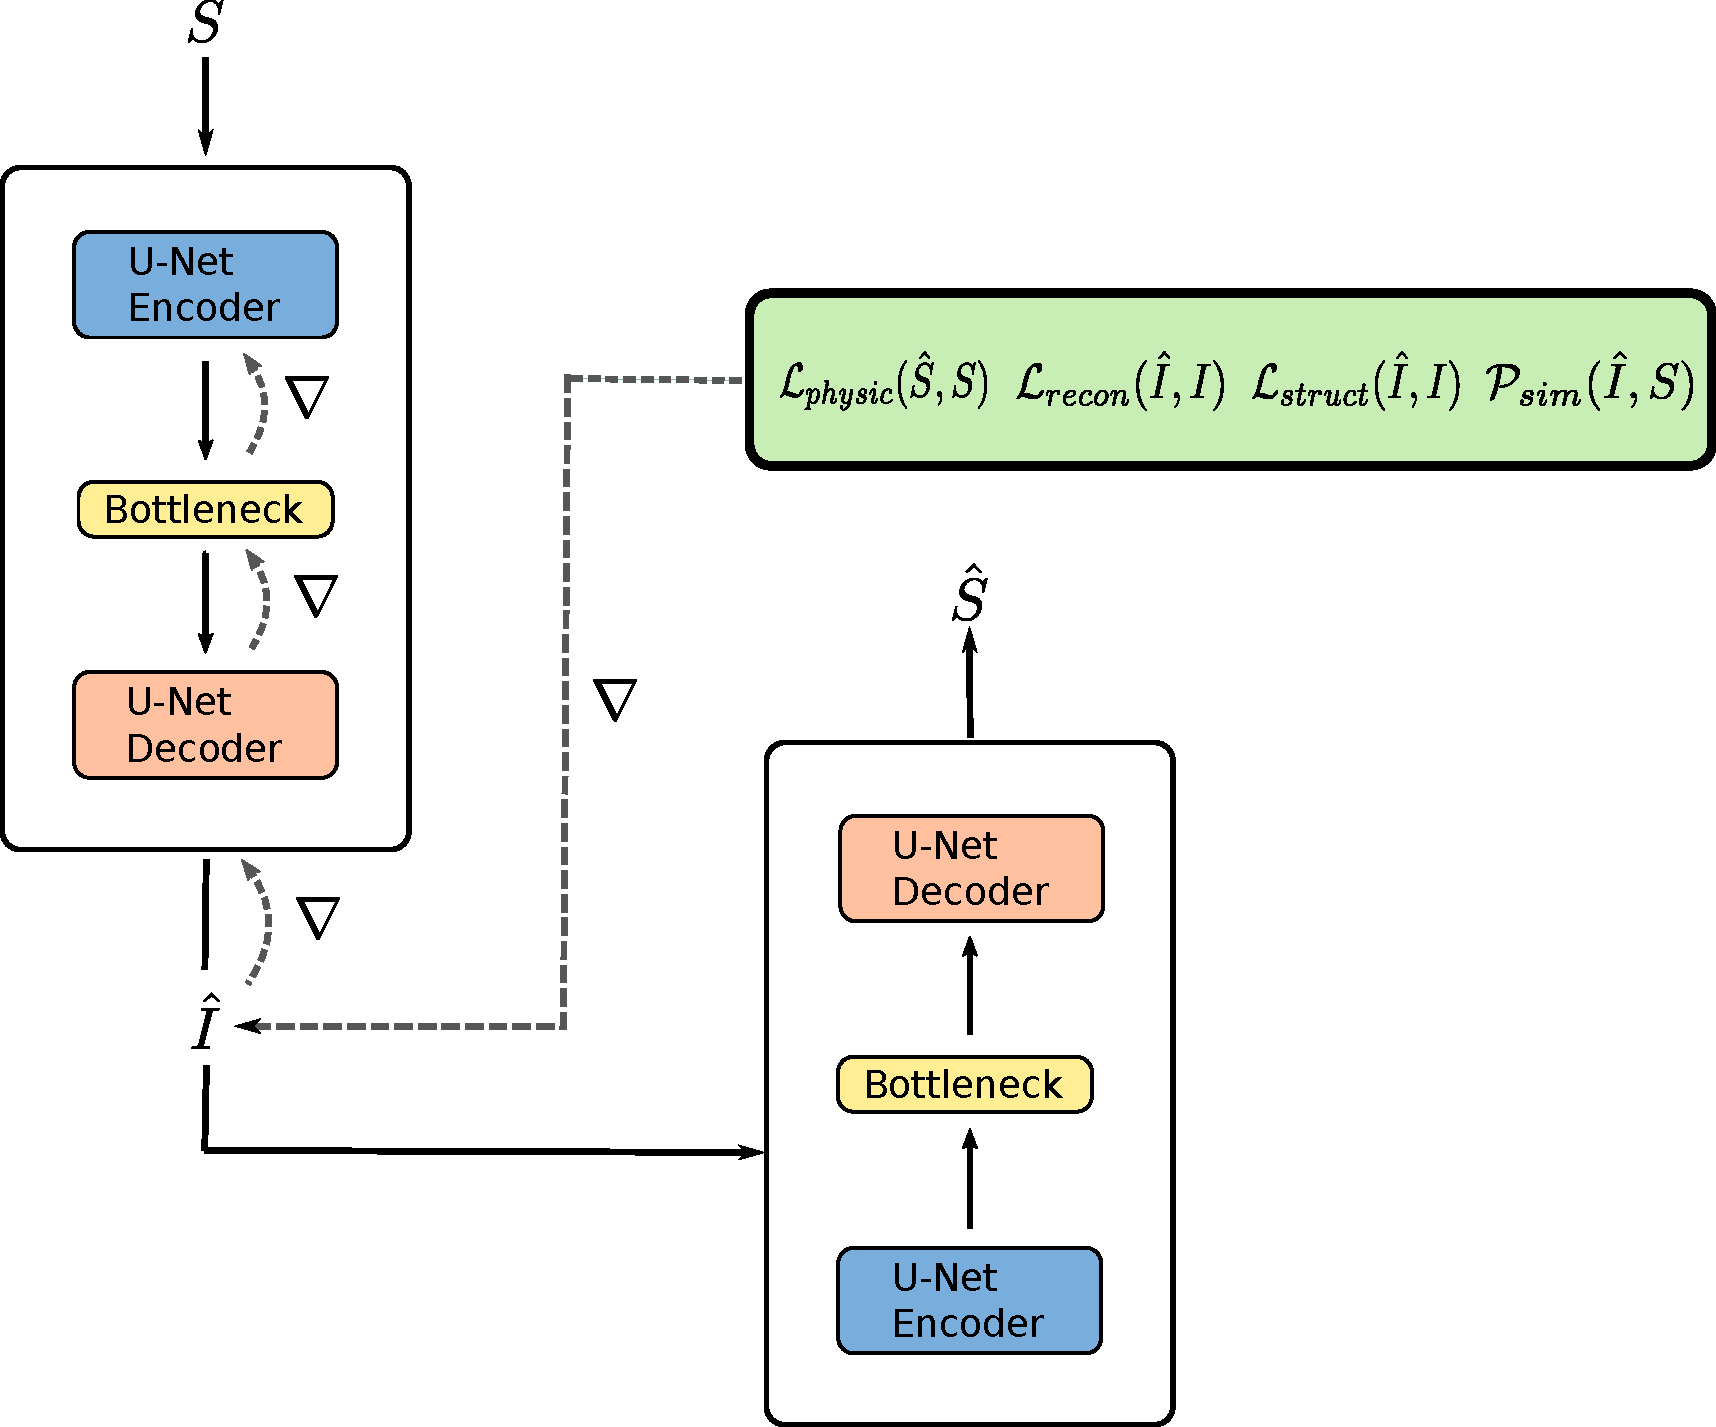
\includegraphics[width=0.8\textwidth]{Images/arq.pdf}
    \caption{Arquitectura de la red propuesta. La red reconstructora se entrena para aprender el mapeo directo de señales acústicas a imágenes fotoacústicas. La red supervisora se entrena para emular el proceso físico de generación de señales acústicas a partir de una imagen dada. Durante el proceso de fine-tuning, la red reconstructora se entrena para generar imágenes que, al ser procesadas por la red supervisora, produzcan señales acústicas consistentes con las mediciones originales.}
    \label{fig:fine-tuning}
\end{figure}

La red reconstructora tiene como objetivo principal transformar las señales acústicas medidas ($S$) en imágenes fotoacústicas ($\hat{I}$), mientras que la red supervisora actúa como un evaluador físico, aprendiendo a simular el proceso de generación de señales acústicas a partir de una imagen dada. La clave de este enfoque es el entrenamiento en dos fases: un preentrenamiento individual de cada red seguido de un proceso de fine-tuning que incorpora la supervisión física.

\subsection{Arquitectura del Sistema}

Ambas redes siguen una arquitectura U-Net modificada que consiste en:
\begin{itemize}
    \item Un codificador (Encoder) que extrae características relevantes de la entrada
    \item Un cuello de botella (Bottleneck) que comprime la información
    \item Un decodificador (Decoder) que reconstruye la salida deseada
\end{itemize}

\subsection{Preentrenamiento Individual}

El preentrenamiento se realiza de manera independiente para cada red, estableciendo las capacidades básicas necesarias para el proceso de fine-tuning posterior.

\subsubsection{Red Reconstructora}
La red reconstructora se entrena para aprender el mapeo directo de señales acústicas a imágenes fotoacústicas. Durante esta fase, la red optimiza:

\begin{equation}
    \mathcal{L}_A = \text{MSE}(\hat{I}, I)
\end{equation}

donde $\hat{I}$ es la imagen reconstruida y $I$ es la imagen objetivo. Esta pérdida asegura que la red aprenda a generar reconstrucciones visualmente precisas.

\subsubsection{Red Supervisora}
La red supervisora se entrena para aproximar el proceso físico de generación de señales acústicas. Este proceso puede ser modelado como:

\begin{equation}
    S = \mathcal{F}(I) + \epsilon
\end{equation}

donde $\mathcal{F}$ representa una aproximación del operador físico de propagación fotoacústica. En la práctica, este operador encapsula las complejas relaciones descritas por las ecuaciones de onda fotoacústica presentadas en la sección \ref{sec:fundamentos}. La red neuronal actúa como un aproximador universal de esta función, aprendiendo a mapear las imágenes a sus correspondientes señales acústicas sin necesidad de resolver explícitamente las ecuaciones diferenciales parciales subyacentes. El término $\epsilon$ modela tanto el ruido del sistema como los errores de aproximación inherentes a este enfoque.

La red optimiza:
\begin{equation}
    \mathcal{L}_B = \text{MSE}(\hat{S}, S)
\end{equation}

donde $S_{pred}$ es la señal acústica predicha por la red y $S_{true}$ es la señal acústica medida. Este entrenamiento permite a la red supervisora aprender implícitamente las características físicas del proceso fotoacústico, actuando como un simulador aprendido del sistema físico.

\subsection{Flujo de Datos}

Durante el proceso de reconstrucción, los datos fluyen de la siguiente manera:
\begin{enumerate}
    \item La señal acústica $S$ ingresa a la red reconstructora
    \item La red reconstructora genera una imagen reconstruida $\hat{I}$
    \item Esta imagen es procesada por la red supervisora para generar una señal acústica predicha $\hat{S}$
    \item Las diferentes pérdidas se calculan comparando las salidas con los valores objetivo
\end{enumerate}

Este diseño permite que la red reconstructora aprenda no solo de la comparación directa con las imágenes objetivo, sino también de la retroalimentación proporcionada por la red supervisora a través de la consistencia física de las señales acústicas generadas.

\subsection{Fine-tuning con Supervisión Física}

El proceso de fine-tuning se realiza sobre la red reconstructora previamente entrenada, incorporando un mecanismo de supervisión física a través de la red supervisora. Este proceso está diseñado para asegurar que las imágenes reconstruidas no solo sean visualmente precisas, sino que también mantengan consistencia con las propiedades físicas del sistema fotoacústico.

La estructura del fine-tuning involucra cuatro términos de pérdida complementarios:

\begin{equation}
    \mathcal{L}_{total} = \lambda_{1} \mathcal{L}_{recon} + \lambda_{2} \mathcal{L}_{physics} + \lambda_{3} \mathcal{L}_{struct} + \lambda_{4} \mathcal{P}_{sim}
\end{equation}

donde:

\begin{itemize}
    \item $\mathcal{L}_{recon}$ mide la discrepancia entre la imagen reconstruida $\hat{I}$ y la imagen objetivo $I$:
    \begin{equation}
        \mathcal{L}_{recon} = \text{MSE}(\hat{I}, I)
    \end{equation}
    
    \item $\mathcal{L}_{physics}$ evalúa la consistencia física comparando la señal acústica predicha $\hat{S}$ con la señal real $S$:
    \begin{equation}
        \mathcal{L}_{physics} = \text{MSE}(\hat{S}, S)
    \end{equation}
    
    \item $\mathcal{L}_{struct}$ preserva las características estructurales de la imagen:
    \begin{equation}
        \mathcal{L}_{struct} = 1 - \text{SSIM}(\hat{I}, I)
    \end{equation}
    
    \item $\mathcal{P}_{sim}$ es un término de penalización que previene que la red tome atajos durante el aprendizaje:
    \begin{equation}
        \mathcal{P}_{sim} = \text{cos\_similarity}(\hat{I}, S)
    \end{equation}
\end{itemize}

Los coeficientes $\lambda_i$ ponderan la contribución de cada término en la pérdida total. Durante el fine-tuning, la red supervisora se mantiene con sus pesos congelados, actuando como un evaluador fijo de la consistencia física de las reconstrucciones. Esta red toma la imagen reconstruida $\hat{I}$ y genera una predicción de la señal acústica $\hat{S}$ que debería producir dicha imagen.

El término $\mathcal{L}_{physics}$ es particularmente importante ya que fuerza a la red reconstructora a generar imágenes que, cuando son procesadas por la red supervisora, producen señales acústicas consistentes con las mediciones originales. Esto asegura que la reconstrucción no solo sea visualmente precisa ($\mathcal{L}_{recon}$ y $\mathcal{L}_{struct}$) sino que también respete las propiedades físicas del sistema fotoacústico.

El término de penalización $\mathcal{P}_{sim}$ es crucial para evitar que la red tome atajos en el proceso de aprendizaje. Sin esta penalización, la red podría tender a generar imágenes que son similares a las señales de entrada, lo cual produciría señales acústicas similares a las originales (minimizando $\mathcal{L}_{physics}$) pero no representaría una reconstrucción válida del objeto original.

Este enfoque de fine-tuning permite que la red reconstructora refine sus predicciones incorporando conocimiento físico del sistema, mientras mantiene la calidad visual y estructural de las reconstrucciones. La combinación de los diferentes términos de pérdida asegura un balance entre la fidelidad de la reconstrucción y la consistencia física del resultado.
